% !TeX spellcheck = en_US
\documentclass[a4paper,12pt]{article}

\usepackage{fullpage}
\usepackage{fourier}
\usepackage{amsmath}
\usepackage{color}
\usepackage{graphicx}
\usepackage{titlesec}

\titleformat{\subsection}[hang]{\large\bfseries}{\alph{subsection})\quad}{0pt}{}

\newcommand{\twodo}[1]{\textcolor{red}{\textbf{todo:} #1}}

\title{\textbf{Exercises for Image Processing 1}\\Problem Sheet 3}
\author{Tim Dobert\\6 \and Konstantin M\"ollers\\6313136}

\begin{document}
	\maketitle
	
	\section{Perspective Transforms}
	
	\subsection{Straight Line Projection}
	
	A straight line in a 3D scene can be described by the following formula:
	
	\begin{align}\label{eqn:1} \vec{t} = \vec{p} + r \cdot \vec{d},\end{align}
	where $\vec{p}$ is a position vector and $\vec{d}$ is a direction vector. Every possible point on the line $\vec{t}$ can be reached by finding the appropriate $r$.
	
	Furthermore, we can split the equation~\ref{eqn:1} into its components:
	\begin{align}
		t_x &= p_x + r \cdot d_x \\
		t_y &= p_y + r \cdot d_y \\
		t_z &= p_z + r \cdot d_z.
	\end{align}
	
	If we now perform the projection, we obtain the following formulas:
	\begin{align}
		\label{eqn:2} t'_{x} &= t_x \cdot \frac{f}{t_z} \\
		\label{eqn:3}t'_{y} &= t_y \cdot \frac{f}{t_z}\\
		t'_{z} &= f.
	\end{align}
	
	From equations \ref{eqn:2} and \ref{eqn:3} we can conclude a straight line vector specification for a 2D scene:
	
	\begin{align}\label{eqn:4} \vec{s} = \vec{0} + \frac{f}{t_z} \cdot \binom{t_x}{t_y}.\end{align}
	
	Because we were able to construct a 2D straight line formula from any 3D one, we have shown that the obtained 2D projection stays a straight line. $\square$
	
	\subsection{Parallel Line Projection}
	
	Regarding perspective projection, parallel lines meet each other in the vanishing point, which concludes in the loss of parallelism of the former. If you use an \textbf{Orthographic projection} instead, the Z-axis of a Cartesian coordinate system is just pointing in some diagonal direction, no matter which X or Y position is applied. So, in that projection, all lines which are parallel in the real world will also be parallel in the orthographic projected world.

	
	\subsection{Sphere Projection}
	
	Given a sphere in the scene, we can visualize the set of points which connect the optical center of the camera to the edges of the visible hemisphere of the sphere as being a geometrical cone with the same radius and the top angle lying on the center. This cone is sliced by the image plane and rendered 2-dimensional exactly how the sphere is represented on the resulting picture.
	
	So given a not null focal distance, a normal optical axis to the image plane and a sphere lying on a side of the image plane, the sphere will result in a circle in the image if its center point lies on the optical axis of the camera, thus the geometrical cone is then sliced by a plane parallel to its base, while in any other case the sphere will be an ellipse. You can see the effect in the following image.
	
	\begin{figure}[h!]
		\centering
		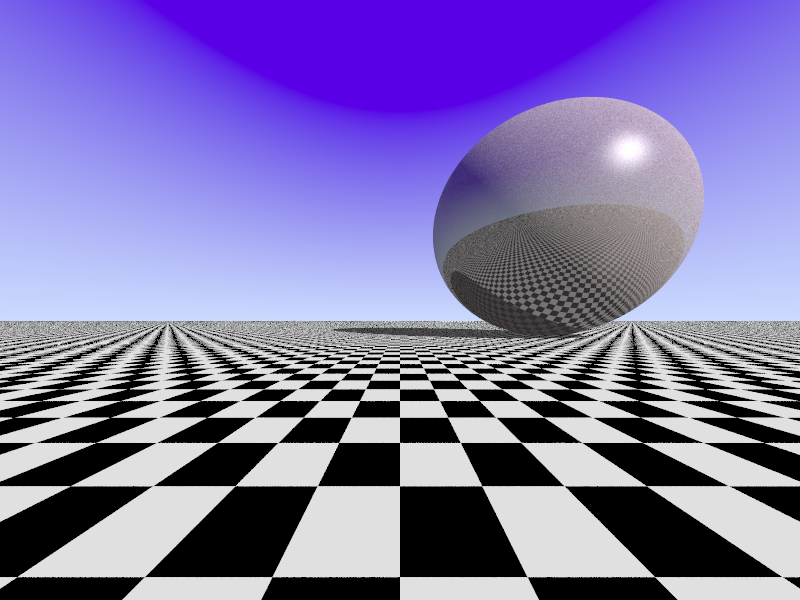
\includegraphics[width=0.7\textwidth]{E03.png}
		\caption{Sphere rendered with perspective projection in POV-Ray.}
	\end{figure}
	
	
\end{document}
